% THIS IS SIGPROC-SP.TEX - VERSION 3.1
% WORKS WITH V3.2SP OF ACM_PROC_ARTICLE-SP.CLS
% APRIL 2009
%
% It is an example file showing how to use the 'acm_proc_article-sp.cls' V3.2SP
% LaTeX2e document class file for Conference Proceedings submissions.
% ----------------------------------------------------------------------------------------------------------------
% This .tex file (and associated .cls V3.2SP) *DOES NOT* produce:
%       1) The Permission Statement
%       2) The Conference (location) Info information
%       3) The Copyright Line with ACM data
%       4) Page numbering
% ---------------------------------------------------------------------------------------------------------------
% It is an example which *does* use the .bib file (from which the .bbl file
% is produced).
% REMEMBER HOWEVER: After having produced the .bbl file,
% and prior to final submission,
% you need to 'insert'  your .bbl file into your source .tex file so as to provide
% ONE 'self-contained' source file.
%
% Questions regarding SIGS should be sent to
% Adrienne Griscti ---> griscti@acm.org
%
% Questions/suggestions regarding the guidelines, .tex and .cls files, etc. to
% Gerald Murray ---> murray@hq.acm.org
%
% For tracking purposes - this is V3.1SP - APRIL 2009

\documentclass{acm_proc_article-sp}

\begin{document}

\title{Ramp it up! Action based guide for \\creating accessible websites\titlenote{A large format version of this poster is available at the author's website at \texttt{terracoda.net}}}
%
% You need the command \numberofauthors to handle the 'placement
% and alignment' of the authors beneath the title.
%
% For aesthetic reasons, we recommend 'three authors at a time'
% i.e. three 'name/affiliation blocks' be placed beneath the title.
%
% NOTE: You are NOT restricted in how many 'rows' of
% "name/affiliations" may appear. We just ask that you restrict
% the number of 'columns' to three.
%
% Because of the available 'opening page real-estate'
% we ask you to refrain from putting more than six authors
% (two rows with three columns) beneath the article title.
% More than six makes the first-page appear very cluttered indeed.
%
% Use the \alignauthor commands to handle the names
% and affiliations for an 'aesthetic maximum' of six authors.
% Add names, affiliations, addresses for
% the seventh etc. author(s) as the argument for the
% \additionalauthors command.
% These 'additional authors' will be output/set for you
% without further effort on your part as the last section in
% the body of your article BEFORE References or any Appendices.

\numberofauthors{1} %  in this sample file, there are a *total*
% of EIGHT authors. SIX appear on the 'first-page' (for formatting
% reasons) and the remaining two appear in the \additionalauthors section.
%
\author{
% You can go ahead and credit any number of authors here,
% e.g. one 'row of three' or two rows (consisting of one row of three
% and a second row of one, two or three).
%
% The command \alignauthor (no curly braces needed) should
% precede each author name, affiliation/snail-mail address and
% e-mail address. Additionally, tag each line of
% affiliation/address with \affaddr, and tag the
% e-mail address with \email.
%
% 1st. author
\alignauthor
Taliesin L. Smith\titlenote{The author is also an Instructional Design Specialist at Memorial University, St.John's, Newfoundland Labrador}\\
       \affaddr{MDes. (Candidate) Inclusive Design, }\affaddr{OCAD University, }\\
       \affaddr{Toronto, Ontario, Canada}\\
       \email{talilief@gmail.com}
}
\date{19 January 2015}

\maketitle
\begin{abstract}
Presented here is an action-based guide to creating accessible websites.

The simplified action-based techniques focus on making accessibile design decision that take place throughout a project. By focusing on accessibility rather than compliance we hope this guide will help teams create sites that are perceivable, operable, understandable and robust. The POUR [0] principles of the Web Content Accessibility Guidelines (WCAG 2.0) are what all the other layers aim to achieve. The poster aims to make all members of the web team - designers, developers, writers and project managers more aware of when \& where barriers can slip in. Each stair needs varying amounts of awareness, skill \& resources in order to implement the techniques and build in the \textit{virtual ramp}. Integrating accessibility into our design process brings us closer to a universal web[0].

\end{abstract}

% A category with the (minimum) three required fields and an optionl 4th field 
% \category{H.1.2}{User/Machine Systems}{Human Factors}
%\category{D.2.8}{Software Engineering}{Metrics}[complexity measures, performance measures]
\category{H.1.2}{User/Machine Systems}{Human Factors}
\category{H.5.2}{User Interfaces}{Standardization}
\category{H.5.4}{Hypertext/ Hypermedia}{User issues}
\category{D.2.10}{Design}{Methodologies}

\terms{inclusive design, web accessibility, WCAG, standards} % NOT required for Proceedings

\section{Introduction}
A long term study [7] found low compliance rates with the Web Content Accessibility Guidelines (WCAG), but at the same time, uncovered a growing adherence to \textit{some} criteria. A follow-up study [10] found that at least part of the improved accessibility was a side effect of changes in coding practices, new browser capabilities and concerns over page rankings. In another study [9], \textit{lack of awareness and knowledge of the WCAG} was identified by the participants to be the most significant barrier to web accessibility. These studies show that web teams continue to struggle with correct implementation of the WCAG and suggest that aids that make the guidelines easier to understand and implement could improve web accessibility. This poster intends to do just that, help teams focus on accessible design choices to design \& build in the \textit{virtual ramp}. 

\begin{figure*}
\centering
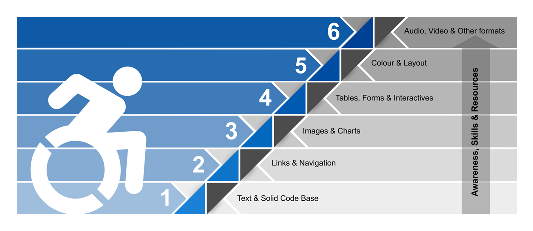
\epsfig{file=stairs-ramp.eps, width=14cm}
\caption{Each content type or design decision represents a stair or potential barrier. The numbers associate each stair with a list of action-based techniques that outline how to build in the \textit{virtual ramp}.}
\end{figure*}

\section{Building in the {\secit Virtual} Ramp}

\subsection{Text \& Solid Structure}

Electronic text-based content is accessible by nature. It can be rendered visually, auditorily and tactilely. Use HTML's built-in semantic structure [1] - headings, lists, quotes - to code meaning directly into your content. Keep the reading level as simple as possible. Define the natural language \& mark language changes. Ensure there is a doctype, charset \& page title in each of your templates for a valid code base. Unique page titles reassures users they are in the right place.

\subsection{Navigation, Links \& Landmarks}
Navigation, links and landmarks, like stepping stones, help you find your way [8]. Use unique self-describing meaningful words for linked text. Leave context changes - pop-ups, new tabs - in the control of the user. Use WAI-ARIA [3] landmark roles, HTML5 landmark tags or skip-navigation links to provide direct access to page content. Design well-planned, consistent navigation as accessible sites also need to be usable.

\subsection{Images \& Charts}
Provide meaningful text alternatives for all content images. The alt attribute is required, but can be left empty, if appropriate in the context. For charts or complex images you may need to link to supplementary content or use the longdesc attribute. The goal of text alternatives is to maintain the meaning of the document whether you can see the image or not.

\subsection{Tables, Forms \& Interactives}
Simplify complex HTML structures such as tables \& forms whenever possible. user interactions wherever possible. Ensure all controls \& interactions are accessible via the keyboard.
\subsubsection{Table}
Table structure conveys meaning about the data within it. Use the rich semantic mark-up available for tables - caption, thead, tfoot, tbody to make data realtionship clear. Appropriately distinguish table header cells from table data cells (th, td) on rows and columns. Do not use tables for layout. They are for tabular data only!

\subsubsection{Forms \& Interactives}
Keep forms simple - don't ask for data you don't need. Use \& associate labels for every form control. Use the button element when you need a button. Group form controls create meaningful organization in forms - legend, fieldset, optgroup. Organizational meaning is good for all users. Design clear error identification \& intuitive error handling by clearly telling the user where they have gone wrong, how to fix the problem and when they have succeeded. Provide reasonable time-outs (think user control). Employ WAI-ARIA [3] to define roles and behaviours that HTML cannot describe. This is particularly important for forms \& interactive structures that use forms (e.g. games, quizzes, etc.).

Note: most legal cases have happened around in-accessible tables \& forms [0].

\subsection{Colour \& Layout}
CSS is the standard to use for presentation. Use it correctly to maintain global control of your layout \& design. Using CSS \& HTML together properly is best method in making your content accessible \& easier to maintain. Choose colours wisely \& test for sufficient contrast ratios. Avoid confusing colours [0]. Don't rely on colour alone for meaning.

\subsection{Audio, Video \& Other formats}
Like images multimedia need text alternatives to be made accessible. Controls for media must be operable by the keyboard. Think user control - do not auto-playing anything. Provide captions for video \& transcripts for audio. In some cases (e.g. talking heads, interviews) transcripts are make better sense than captions. For ultimate accessibilty describe video when the meaning cannot be understood by the soundtrack alone. For other formats, such as PDF or Word documents, first ask is there a reason not to use HTML? When HTML is not an option, one must follow the same principles (WCAG 2.0) to make content in Word documents and PDFs accessible. PDFs must be tagged to be accessible [0].

\section{Conclusions}
 It is well documented that making the choice for inclusion has beneficial side effects []. In the case of an accessible website it will be easier to find, load faster, be easier to maintain, change \& customize. It will work better with mobile devices, lasts longer \& be usable by more people - all of these are good for business \& contribute to a better bottom line. Just like accessibility ramps and curbcuts benefit more than just people in wheelchairs, accessible websites benefit many more than the intended audience.
%\end{document}  % This is where a 'short' article might terminate

%ACKNOWLEDGMENTS are optional
\section{Acknowledgments}
Special thanks to the {\it Accessible Icon Project} for the icon and Amita Pharshy and Andrea Quigley for their comments.

%REFERENCES as a SECTION
\section{References}
\begin{itemize}
%\item[1] (2013) Semantic Structure. WebAIM.org. \\http://webaim.org/techniques/semanticstructure/
%\item[1] Don't reapeat yourself. Wikipedia.\\http://wikipedia.org/wiki/Don't\_repeat\_yourself
\item[2] Brewer, C. Harrower, M. \& Pennsylvania State University. Color Brewer 2.0 http://colorbrewer2.org/
\item[3] Clark, J. (2003). {\it Building accessible websites.} Indianapolis: New Riders.
\item[6] Clark, J. (2005). Facts and opinions about PDF accessibility. {\it A List Apart.}\\http://alistapart.com/article/pdf\_accessibility
\item[4] Hanson, V., \& Richards, J. (2013). Progress on website accessibility? {\it ACM Transactions on the Web, 7}(1).
\item[5] Horton, S. \& Quesenbery, W. (2014). {\it A Web for everyone: Designing accessible user experiences.} Brooklyn: Rosenfeld Media.
\item[0] Jacobs, S. (1999). Section 255 of the Telecommunications Act of 1996: Fueling the Creation of New Electronic Curbcuts.\\http://www.accessiblesociety.org/topics/technolog/eleccurbcut.htm 
\item[6] Lazar, J., Dudley-Sponaugle, A. \& Greenidge, K. D. (2004). Improving web accessibility: as study of web master perceptions. {\it Computers in Human Behavior, 20}(2). pp 269-288.
\item[7] Monsebraaten, L. (2012 Mar 31). Toronto woman wins  second victory ordering governemnt websites accessible to the blind. {\it Toronto Star.} http://www.thestar.com/
\item[8] Richards, J. T., Montague, K. \& Hanson, V. L., (2012). Web Accessibility as a Side Effect, {\it ASSETS '12 Proceedings of the 14th international ACM SIGACCESS conference on Computers and accessibility}. pp 79-86.
\item[0] CSS. http://www.w3.org/TR/CSS
\item[0] WAI-ARI. http://www.w3.org/TR/wai-aria
\item[0] WCAG 2.0. http://www.w3.org/TR/WCAG20
%\item[0] WCAG Samurai: http://www.wcagsamurai.org
%\item[0] WCAG 1.0: http://www.w3.org/TR/WAI-WEBCONTENT		
\end{itemize}
%
% The following two commands are all you need in the
% initial runs of your .tex file to
% produce the bibliography for the citations in your paper.
\bibliographystyle{abbrv}
\bibliography{sigproc}  % sigproc.bib is the name of the Bibliography in this case
% You must have a proper ".bib" file
%  and remember to run:
% latex bibtex latex latex
% to resolve all references
%
% ACM needs 'a single self-contained file'!
%
\balancecolumns
% That's all folks!
\end{document}
